\chapter{Method}\label{cha:method}

\section{Datasets}

The experiments in this thesis use both uniform-grid and non-uniform
datasets. For each dataset, the goal of this section is to describe the
underlying physical problem, the mapping learned by the model, the data
source, and the aspects of the dataset that are relevant for
interpreting the results. Dataset-specific implementation details are
included only when they affect the conclusions drawn later in the
thesis. In particular, the full generation procedure for the Navier-Stokes dataset generated in this work is deferred to Appendix~\ref{navier-details}. Unless stated otherwise, all datasets were split into training, validation, and test sets using an 80/10/10 split. All datasets but one are given in dimensionless units. The exception is the high-temperature gas-cooled reactor (HTGR) column dataset, which is given in degrees Celsius and centimeters.

\subsection{Uniform-Grid Datasets}

The discretization invariance experiments on regular grids use two
datasets: a Navier-Stokes dataset generated in this work and a Darcy flow
dataset obtained from prior work.

\subsubsection{Navier-Stokes}\label{navier-stokes}

\begin{figure}
    \centering
    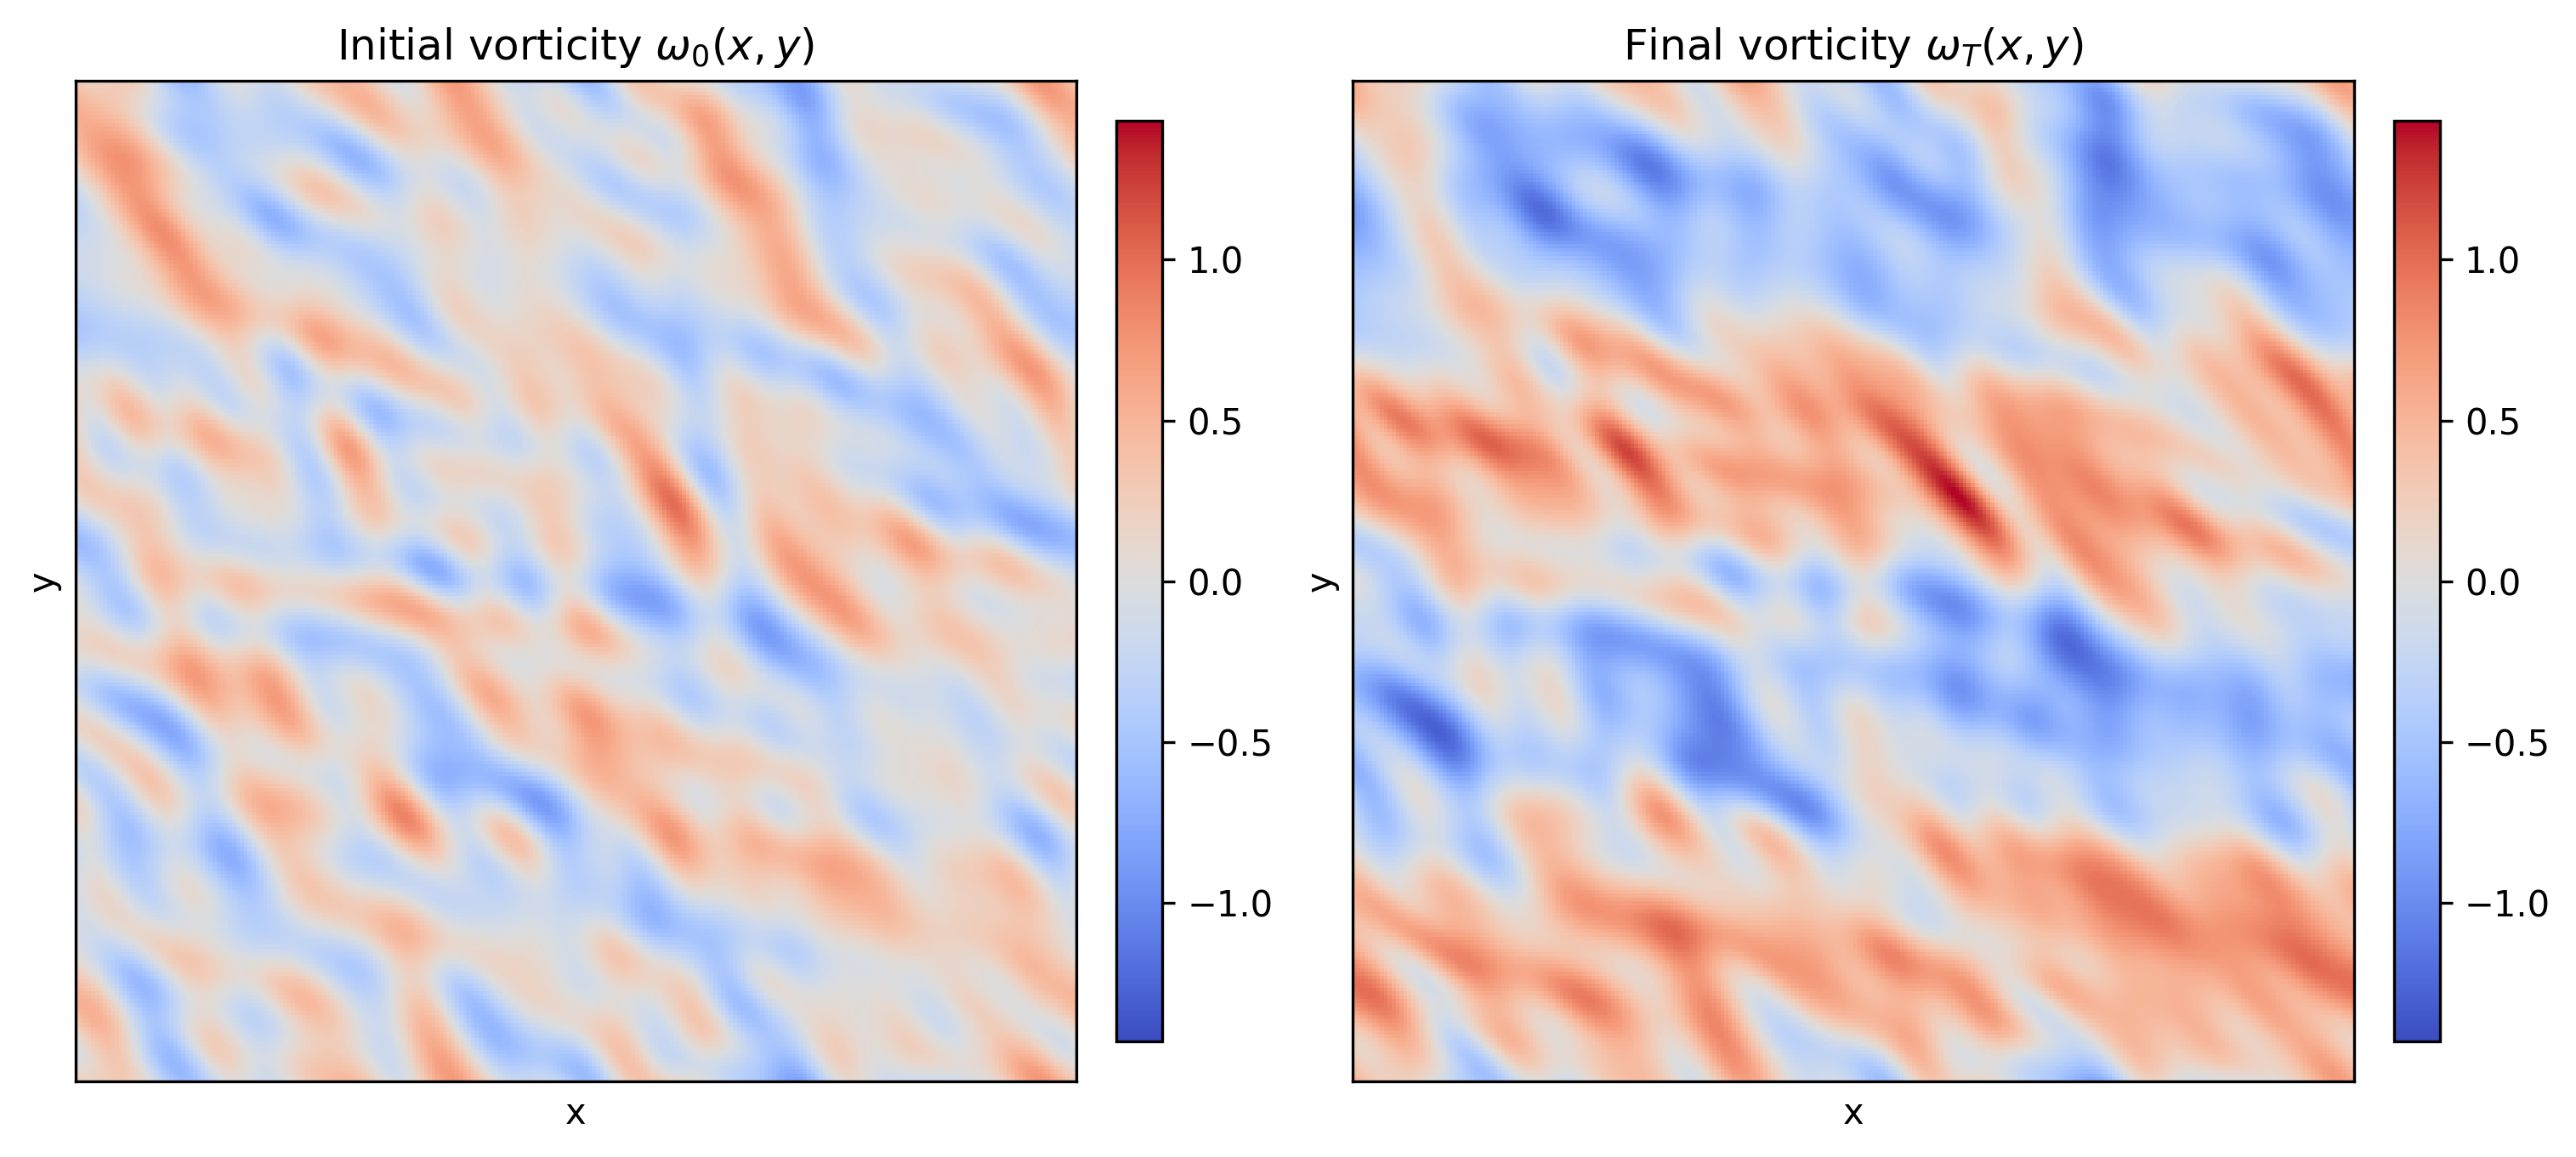
\includegraphics[width=0.8\textwidth]{figures/navier_input_output.png}
    \caption{\label{fig:navier} Initial and final vorticity fields for a sample from the Navier-Stokes dataset.}
\end{figure}

For the regular-grid experiments, we use a two-dimensional Navier-Stokes dataset on the unit square. The Navier-Stokes equations are among the fundamental equations of fluid dynamics and arise in many areas of physics and engineering, including atmospheric and oceanic flows, aerodynamics, and industrial transport processes. The dataset is formulated and solved in vorticity form, with governing equation:


\begin{equation}
    \partial_t \omega + u \cdot \nabla \omega = \nu \Delta \omega + f,
\end{equation}

where $\omega$ denotes the vorticity field, $u$ the incompressible velocity field, $\nu$ the viscosity, and $f$ an external forcing term. The learning task considered in this thesis is not a pressure or velocity prediction problem, but an operator mapping from an initial vorticity field to a later vorticity field. The input to the model is the initial vorticity field $\omega(\cdot,0)$, and the output is the vorticity field at a later time $\omega(\cdot,T)$. An example input-output pair is shown in Figure~\ref{fig:navier}.

The dataset consists of 1000 samples generated at a resolution of $256 \times 256$. Between samples, the viscosity and forcing remain fixed, while the initial vorticity field is varied. Further dataset details and explanation of the data-generation procedure are provided in Appendix~\ref{navier-details}.

\subsubsection{Darcy flow}\label{darcy-flow}

Also used for the uniform-grid experiments is the Darcy flow dataset introduced by Li et al. \cite{li2021fno}. 
In this benchmark, the task is to learn the solution operator of a steady-state two-dimensional Darcy flow problem
on the unit square, governed by the following PDE:

\begin{equation}
    -\nabla \cdot (a(x)\nabla u(x)) = f(x), \qquad x \in (0,1)^2,
\end{equation}
\begin{equation}
    u(x) = 0, \qquad x \in \partial(0,1)^2,
\end{equation}

\begin{figure}
    \centering
    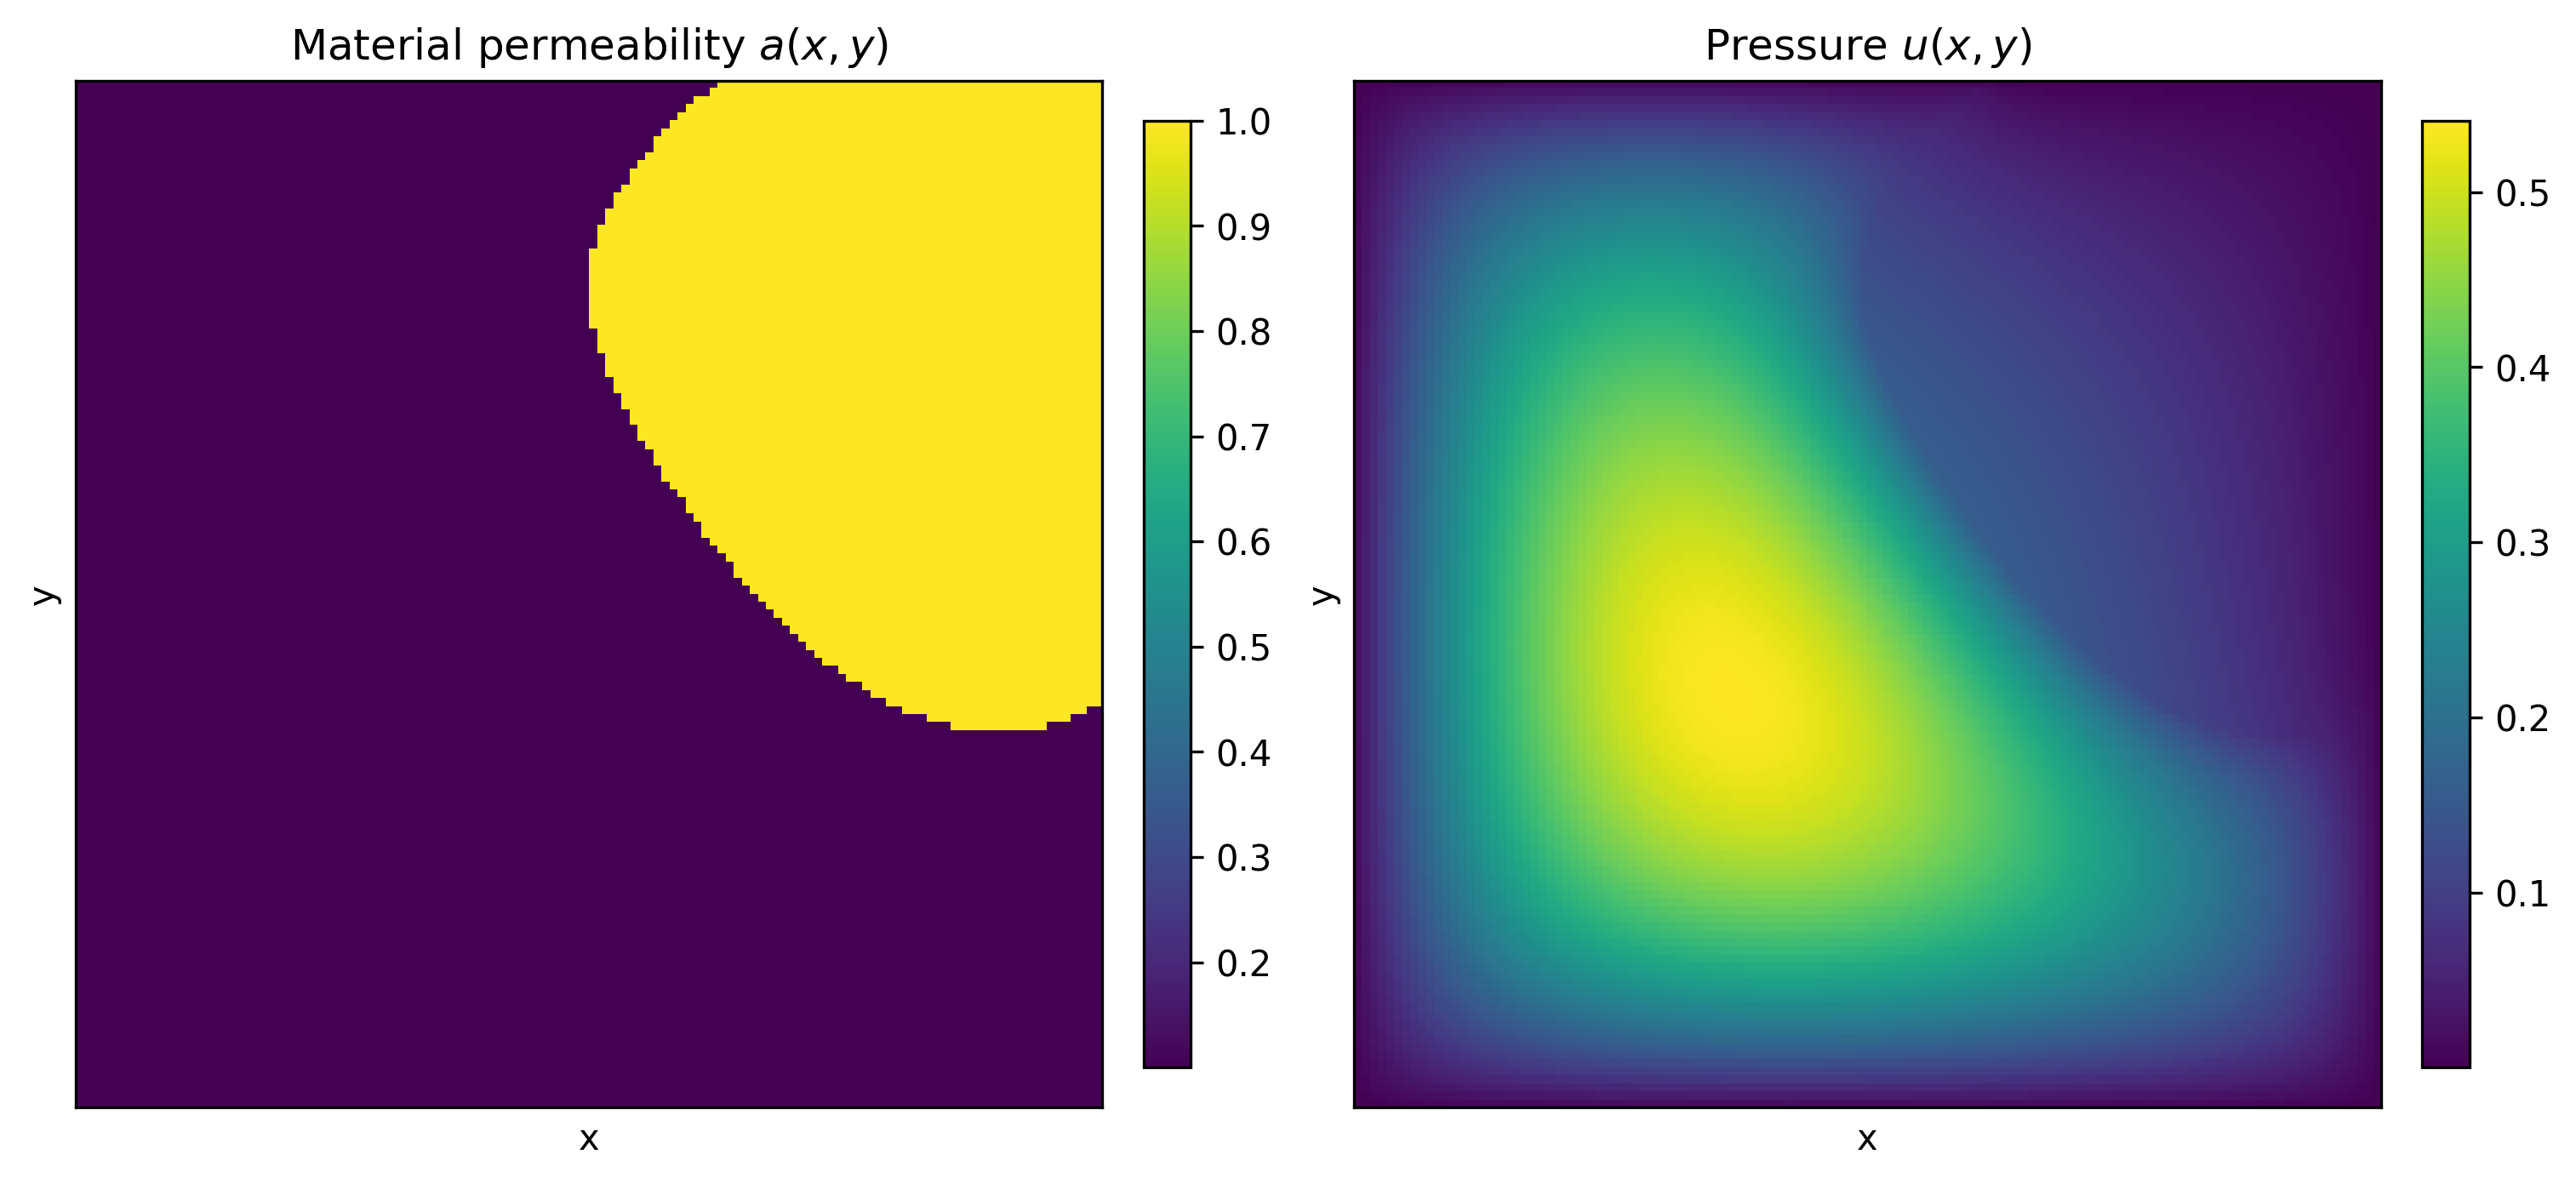
\includegraphics[width=0.9\textwidth]{figures/darcy_input_output.png}
    \caption{\label{fig:darcy} Example of an input diffusion coefficient field \(a(x,y)\) and the resulting pressure
    field \(u(x,y)\) with Dirichlet boundary conditions.}
\end{figure}

The input is a spatially varying permeability field \(a(x)\), and the output is the corresponding pressure field \(u(x)\) under a prescribed forcing term and Dirichlet boundary conditions. An example
 input-output mapping can be seen in figure \ref{fig:darcy}. Between samples, $f(x)$ is kept constant while the $a(x)$ is varied. This PDE has many applications within physics and engineering, including drainage and irrigation in agricultural soils and fluid migration around nuclear waste repositories \cite{darcyapplications}. For this 
  thesis, the Darcy flow dataset serves as a regular-grid benchmark for evaluating the performance of FNO and CNO 
  across discretizations. This dataset was selected because it provides a comparatively smooth benchmark, 
  complementing the more irregular and turbulent behavior of the Navier-Stokes dataset discussed in Section~\ref{navier-stokes}. Using both datasets makes it possible to evaluate model performance under qualitatively different solution regimes. The dataset contains 10000 samples at a resolution of 128$\times$128.



\subsection{Non-Uniform Datasets}\label{non-uniform-datasets}

The experiments on irregular domains primarily use two datasets: an incompressible Navier\hyp{}Stokes
dataset modeling flow past a cylinder and a nuclear engineering
dataset consisting of temperature profiles for a single high temperature gas-cooled reactor (HTGR) column.

\subsubsection{Incompressible Navier-Stokes flow past a cylinder}\label{cylinder-flow-dataset}


The first non-uniform benchmark is an incompressible Navier-Stokes dataset
describing fluid flow past a cylinder. This dataset was used in prior
work on operator learning for PDEs and is included here because it
provides a fluid-dynamics test case on a geometry that is not naturally
aligned with a regular grid \cite{calm-pde, pfaff-datasets}.

The dataset describes two-dimensional incompressible flow with velocity
$\mathbf{v}$ and pressure $p$, governed by:

\begin{equation}
    \nabla \cdot \mathbf{v} = 0,
\end{equation}
\begin{equation}
    \rho_0 \left(\partial_t \mathbf{v} + \mathbf{v} \cdot \nabla \mathbf{v}\right) + \nabla p
    = \mu \nabla^2 \mathbf{v},
\end{equation}

\begin{figure}
    \centering
    \makebox[\textwidth][c]{%
        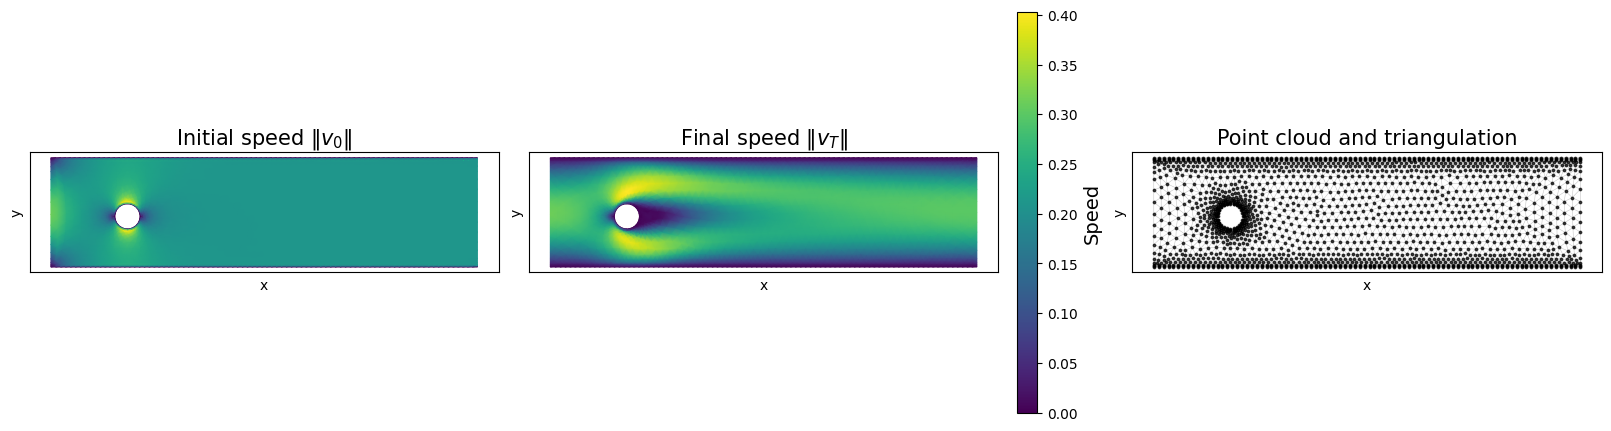
\includegraphics[width=1.1\textwidth]{figures/cylinder_flow_input_output.png}%
    }
    \caption{Example initial and final states
    for the incompressible flow past a cylinder dataset, shown on the
    irregular geometry together with the underlying point cloud. While the model is tasked with predicting the $v_x$ and $v_y$ components of the velocity field, these plots display the speed $\lVert \mathbf{v} \rVert$.}
    \label{fig:cylinder-flow}
\end{figure}

where $\rho_0$ is the constant density and $\mu$ the viscosity. The
domain consists of a channel containing a cylindrical obstacle, with the
cylinder position and radius varying between samples.

The prediction task is to learn a mapping from the initial pressure and velocity fields to the final velocity field, while
accounting for the fact that changes in cylinder size and location lead
to different corresponding flow patterns. In the experiments of this
thesis, the model is trained to predict only the horizontal and vertical
velocity components; pressure is not included in the target.

This dataset is particularly relevant for Geo-FNO because it is defined on a non-uniform spatial discretization rather than a regular Cartesian grid. An example initial-final pair is shown in Figure~\ref{fig:cylinder-flow}. The dataset uses a predefined train-validation-test split, with 1000 training samples, 100 validation samples, and 100 test samples. Each sample contains between 1700 and 2100 points, depending on the geometry of the sample.

\subsubsection{High-Temperature Gas-Cooled Reactor (HTGR) Column Temperature Dataset}\label{htgr-column-dataset}



The next non-uniform dataset consists of steady-state temperature
profiles for a single column of a prismatic core
HTGR. This dataset is included because it provides a first
application-oriented test case for Geo-FNO in a nuclear engineering
setting. Unlike the public benchmark datasets considered earlier, the
data was produced as part of ongoing work by a colleague within the Reactor Physics and Nuclear Materials (RPNM) group of Delft University of Technology.

Physically, the dataset describes the temperature distribution within a
three-dimensional reactor column. For each case, a constant boundary
temperature is imposed and a coupled neutronics-thermohydraulics
calculation is performed until a steady state is reached. The transient
evolution toward this steady state is not included in the dataset; only
the final steady-state temperature fields are used. The use of a fixed
boundary temperature is a simplifying assumption, since in a realistic
reactor system the boundary temperature would itself change as the system
evolves. This simplification was made to produce a controlled dataset
within the time constraints of the project.


The spatial sampling locations lie on an irregular mesh that is shared across all samples. Along the axial direction, the column is quantized into 17 distinct \(z\)-levels. In this thesis, the three-dimensional column data is reformulated as a slice-wise two-dimensional prediction problem: each horizontal slice at a given \(z\)-level is treated as one sample, and the axial coordinate \(z\) is provided as an input parameter to the model. The imposed boundary temperature ranges from \(300\,^{\circ}\mathrm{C}\) to \(1000\,^{\circ}\mathrm{C}\) in steps of \(1\,^{\circ}\mathrm{C}\), yielding 701 distinct thermal conditions. This results in a total of \(17\times701=11917\) two-dimensional samples.

\begin{figure}
    \centering
    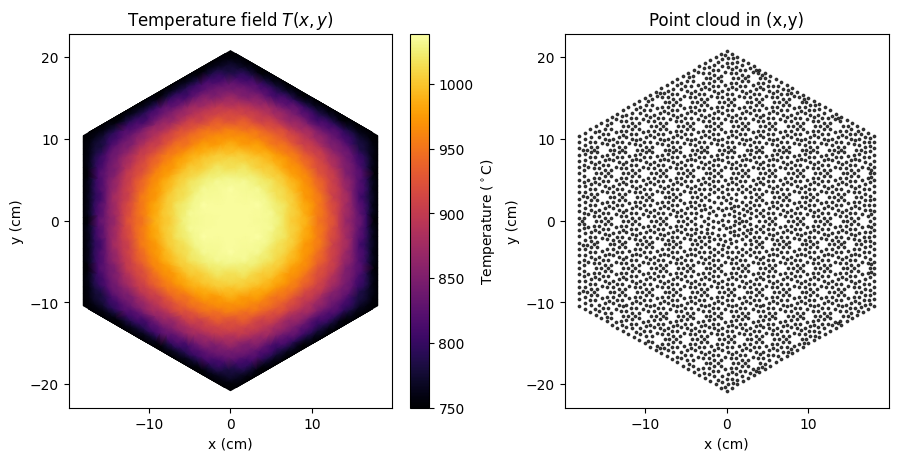
\includegraphics[width=0.8\textwidth]{figures/htgr_column_example.png}
    \caption{\label{fig:htgr-column} Example temperature field from the
    HTGR column dataset for a fixed boundary temperature and selected
    axial layer, shown together with the irregular spatial mesh used for
    sampling. This sample corresponds to an axial level of \(z=30\,\mathrm{cm}\) and a boundary temperature of \(T=750\,^{\circ}\mathrm{C}\).}
\end{figure}

The slices should not be interpreted as independent physical systems. The original temperature fields are generated from a three-dimensional calculation, so axial coupling is already reflected in the resulting temperature profiles. However, the model used in this thesis does not explicitly model interactions between neighboring slices. Instead, it learns a parametric mapping from the imposed boundary temperature and axial coordinate to the temperature distribution on the corresponding horizontal slice.


In the prediction task considered in this thesis, the model receives the
boundary temperature together with a specified $z$-level and predicts
the temperature at all sampled $(x,y)$ locations in the corresponding
horizontal slice. The task can therefore be interpreted as learning a
mapping from the boundary condition and axial position to the
two-dimensional temperature profile within that layer. An example of
such a slice, together with the underlying irregular mesh, is shown in
Figure~\ref{fig:htgr-column}.


\section{Training Setup}

All models are trained in a supervised setting on paired input-output
samples. For each dataset, the available samples were split into training, validation, and test sets. The training set was used to optimize model parameters, while the validation set was used to monitor training and select the final checkpoint. Final reported losses are computed on the test set.

The hyperparameters differ between the uniform-grid and
non-uniform-grid experiments, as well as between datasets. To keep the main text focused on the experimental
design rather than implementation details, hyperparameter settings and training details are given in Appendix~\ref{appendix:hyperparameters}.

Some experiments use feature engineering, meaning that available input variables are transformed before being passed to the model. The purpose is to express the same information in a form that is easier for the network to use, which can improve predictive performance~\cite{feature-engineering}. This is used primarily for the non-uniform datasets, where geometry and low-dimensional parameters play an important role. The specific input representations used for each dataset are described in the corresponding dataset sections.


\section{Uniform-Grid Resolution Transfer Experiments}\label{uniform-experiments}

The uniform-grid experiments are designed to evaluate discretization
invariance by testing how well a model trained at one spatial resolution
generalizes to other resolutions. The Navier-Stokes and Darcy flow
datasets described in \ref{navier-stokes} are used for these experiments. For each dataset, the models are trained at a chosen training resolution and then
evaluated both at the training resolution and at lower and higher
resolutions. This makes it possible to compare performance at the
training resolution with performance after transferring the same trained
model to different spatial resolutions. Both datasets are generated at a single spatial resolution; other resolutions are generated by resampling the data using bicubic interpolation.

For the Navier-Stokes dataset, the models are trained at a resolution of
$192 \times 192$ and evaluated on resolutions from $128 \times 128$ to
$256 \times 256$ in steps of 16 grid points. For the Darcy flow dataset,
the models are trained at a resolution of $96 \times 96$ and evaluated
on resolutions from $64 \times 64$ to $128 \times 128$ in steps of 8
grid points.

Four model variants are compared for each dataset. The first two are FNO
models retaining either 8 or 16 Fourier modes in each spatial direction,
denoted FNO\_k8 and FNO\_k16. The other two are CNO variants. The first is
the regular CNO architecture as outlined in section \ref{sec:cno}, referred to as CNO\_standard. The second is a modified CNO in which the
upsample-nonlinearity-downsample (UND) operation is replaced by a simple pointwise nonlinearity, referred to as CNO\_no\_UND. This operation is one of the architectural changes that distinguishes the CNO from a
U-Net-like architecture and is intended to reduce aliasing effects
introduced by nonlinearities. Comparing the standard and modified CNO
therefore makes it possible to assess the effect of this component in
the resolution-transfer setting.

FNO and CNO handle changes in resolution differently. FNO produces
predictions at the same resolution as the input it is given. In the FNO experiments, evaluation at a resolution \(N \times N\) was performed by first resampling both the input and target fields to \(N \times N\). The resampled input was then passed to the trained FNO, which produces an output on the same grid. This prediction was compared directly with the resampled target field. The CNO, however,
produces predictions on its internal resolution. Therefore, when CNO is
evaluated on an input resolution different from its internal resolution,
the CNO prediction is resampled onto the input resolution before the
error is computed. The target field is resampled to the same resolution,
so that both FNO and CNO are evaluated against target fields on the same
spatial grid. All resampling in these experiments is performed with
bicubic interpolation.





In addition to reporting the mean squared error at each tested resolution, a scalar measure is used to summarize how strongly the loss changes away from the training resolution. Let \(\mathcal{S}\) denote the set of tested resolutions, let \(L_N\) denote the mean squared error at resolution \(N\)\footnote{All uniform-grid experiments in this thesis use square grids. A resolution denoted by \(N\) therefore corresponds to an \(N\times N\) grid, containing \(N^2\) spatial points. This differs from the notation \(n\) used earlier for the total number of grid points.}, and let \(N_{\mathrm{train}}\) denote the training resolution. The discretization variance value is defined as
\begin{equation}
D =
\frac{1}{|\mathcal{S}|}
\sum_{N\in\mathcal{S}}
\left|
\ln(L_N)-\ln(L_{N_{\mathrm{train}}})
\right|.
\end{equation}

The logarithm is used so that the score measures relative, rather than absolute, changes in loss. Equivalently,
\[
\ln(L_N)-\ln(L_{N_{\mathrm{train}}})
=
\ln\left(\frac{L_N}{L_{N_{\mathrm{train}}}}\right),
\]
so \(D\) measures the average multiplicative change in loss relative to the training resolution. For example, a doubling and a halving of the loss contribute equally to \(D\). This makes the score useful for comparing robustness across models whose absolute losses may differ by orders of magnitude.\footnote{In the implementation, a small numerical constant \(\epsilon=10^{-8}\) is added inside the logarithm to avoid numerical issues when losses are very small.}

Lower values of \(D\) indicate that the loss remains closer to the loss at the training resolution across the evaluated resolutions. This score is only a measure of consistency across resolutions, not of absolute model quality. The loss values themselves remain the primary measure of predictive performance, while \(D\) is used only as a quantitative measure of discretization robustness.


\section{Non-Uniform-Grid Geo-FNO Evaluations}\label{non-uniform-experiments}

The non-uniform-grid evaluations use Geo-FNO on the cylinder flow and
HTGR column temperature datasets described in
Section~\ref{non-uniform-datasets}. These evaluations differ from the
uniform-grid resolution transfer experiments in
Section~\ref{uniform-experiments}. Since the spatial samples are given
as point clouds or irregular meshes rather than Cartesian grids, there
is no single resolution parameter equivalent to the grid size $N$ used
in the uniform-grid experiments. The goal is therefore not to measure
resolution transfer, but to evaluate whether Geo-FNO can learn mappings
on irregular spatial data.

For the cylinder flow dataset, the model did not produce meaningful
predictions when it was given only the velocity field on the irregular
mesh. The coordinate transform MLP $\phi^{-1}$ was given the x and y coordinates of the cylinder's center and its radius in the form of the geometric vector $g$. In addition to the horizontal and vertical velocity
components and pressure, each mesh point was also assigned a one-hot encoding of its node
type. The node-type categories distinguish the upper, lower and cylinder boundary nodes, left boundary nodes, right boundary nodes, and interior nodes. This made the location of the obstacle more
explicit in the pointwise input representation, allowing the model to
identify which mesh points lie on or near the cylinder.

For the HTGR column temperature dataset, the raw input consists only of
the boundary temperature $T$ and the axial level $z$. Since this is a
low-dimensional representation of the input conditions, several
alternative representations of $T$ and $z$ were tested through feature engineering. These input
representations and their effect on model performance are discussed in
Appendix~\ref{appendix:htgr-input-engineering}. The best performing representation was used for the results reported in the main text.

Following the discussion in Section~\ref{mesh-free-discretization-invariance}, the non-uniform-grid experiments are treated as held-out evaluations of Geo-FNO on irregular spatial representations. They are not used to compute a mesh-free analogue of the uniform-grid discretization variance value, because the available datasets do not contain controlled refinement families of the same physical samples. The seam artifact observed in early Geo-FNO predictions, and the implementation bug that caused it, are discussed separately in Appendix~\ref{cha:geo-fno-bug-fix}. The results in the main text are reported using the corrected implementation.